\documentclass[11pt]{article}
\usepackage{amsmath,amsbsy,amssymb,verbatim,fullpage,ifthen,graphicx,bm,amsfonts,amsthm,url}
\usepackage{graphicx}
\usepackage{xcolor}
\newcommand{\mfile}[1]  {{\small \verbatiminput{./#1}}} % Jeff Fessler, input matlab file
\newcommand{\tmop}[1]{\ensuremath{\operatorname{#1}}}
%\newcommand*{\qed}{\hfill\ensuremath{\blacksquare}}%
\newcommand{\R}{\mathbb{R}}
\newcommand{\C}{\mathbb{C}}
\newcommand{\Z}{\mathbb{Z}}
\newcommand{\A}{\mathcal{A}}
\newcommand{\minimize}{\operatorname*{minimize\ }}
\newcommand{\maximize}{\operatorname*{maximize}}
\newcommand{\opdet}[1]{\operatorname{\textbf{det}}\left(#1\right)}
\newcommand{\optr}[1]{\operatorname{\textbf{tr}}\left(#1\right)}
\newcommand{\mtx}[1]{\mathbf{#1}}
\newcommand{\vct}[1]{\mathbf{#1}}
\def \lg       {\langle}
\def \rg       {\rangle}
\def \mA {\mtx{A}}
\def \mB {\mtx{B}}
\def \mD {\mtx{D}}
\def \mE {\mtx{E}}
\def \mF {\mtx{F}}
\def \mG {\mtx{G}}
\def \mI {\mtx{I}}
\def \mJ {\mtx{J}}
\def \mL {\mtx{L}}
\def \mU {\mtx{U}}
\def \mS {\mtx{S}}
\def \mV {\mtx{V}}
\def \mW {\mtx{W}}
\def \mLambda {\mtx{\Lambda}}
\def \mSigma {\mtx{\Sigma}}
\def \mX {\mtx{X}}
\def \mY {\mtx{Y}}
\def \mZ {\mtx{Z}}
\def \zero     {\mathbf{0}}
\def \vzero    {\vct{0}}
\def \vone    {\vct{1}}
\def \va {\vct{a}}
\def \vg {\vct{g}}
\def \vm {\vct{m}}
\def \vu {\vct{u}}
\def \vv {\vct{v}}
\def \vw {\vct{w}}
\def \vx {\vct{x}}
\def \vy {\vct{y}}
\def \vz {\vct{z}}
\def \vphi {\vct{\phi}}
\def \vmu {\vct{\mu}}
\def \R {\mathbb{R}}

%\newcommand{\st}{\operatorname*{\ subject\ to\ }}
\usepackage{algorithm,algpseudocode}
\usepackage{xspace}
\usepackage{hyperref}
% Add a period to the end of an abbreviation unless there's one
% already, then \xspace.
\makeatletter
\DeclareRobustCommand\onedot{\futurelet\@let@token\@onedot}
\def\@onedot{\ifx\@let@token.\else.\null\fi\xspace}

\def\eg{\emph{e.g}\onedot} \def\Eg{\emph{E.g}\onedot}
\def\ie{\emph{i.e}\onedot} \def\Ie{\emph{I.e}\onedot}
\def\cf{\emph{c.f}\onedot} \def\Cf{\emph{C.f}\onedot}
\def\etc{\emph{etc}\onedot} \def\vs{\emph{vs}\onedot}
\def\wrt{w.r.t\onedot} \def\dof{d.o.f\onedot}
\def\etal{\emph{et al}\onedot} \def\st{\emph{s.t}\onedot}
\pagestyle{plain}

\title{{\bf Final Exam, CPSC 8420, Fall 2023}} 
\author{\Large\underline{Last Name, First Name}}% put your name in the LastName, FirstName format
\date{\textbf{\Large\textcolor{red}{Due 12/16/2023, Saturday, 5:59PM EST}}} 
%\date{\today}

\begin{document}
\maketitle

\section*{Problem 1 [15 pts]}
Consider the following problem:
\begin{equation}
\min_{\beta} \|\vy-\mX\beta\|^2+\lambda[\alpha\|\beta\|^2_2+(1-\alpha)\|\beta\|_1].
\end{equation}
\begin{enumerate}
	\item Show the objective can be reformulated into a lasso problem, with revised 
	$\hat{\mX}, \hat{\vy}$.\\
	\\Assume we can find
	\begin{align*}
		\|\hat{\vy}-\hat{\mX}\beta\|^2 &= \|\vy-\mX\beta\|^2+\lambda\alpha\|\beta\|^2_2\\
		\implies \|\hat{\vy}\|^2 - 2\hat{\vy}^T\hat{\mX}\beta + \|\hat{\mX}\beta\|^2 &= \|\vy\|^2 - 2vy^T\mX\beta\ + 
		\underbrace{\|\mX\beta\|^2 + \lambda\alpha\|\beta\|^2_2}_{\text{combine these 2 together as }\hat{\mX}}\\
		\implies \hat{\mX} &=  \begin{bmatrix}
			\mX\\
			\sqrt{\lambda\alpha}\vct{I}
			\end{bmatrix}\\
			\hat{\vy} &= \begin{bmatrix}
				\vy\\
				0
				\end{bmatrix}
	\end{align*}

	\item If $\alpha=1/2,\lambda=1$, please derive the closed-form solution by making use of alternating minimization that each time we fix the rest by optimizing one single element in $\beta$. You need randomly generate $\mX, \vy$ and initialize  $\beta_0$, and show the objective decreases monotonically with updates.
	
	\begin{align*}
		&\min_{\beta} \frac{1}{2} \|\hat{\vy}-\hat{\mX\beta}\|^2+\lambda(1-\alpha)\|\beta\|_1\\
		\text{when we try to optimize } \beta_i\\ 
		&\implies  \min_{\beta_i} \frac{1}{2}\|\hat{\vy}- \sum_{j\neq i}\hat{\vx_j}\beta_j-\hat{\vx_i}\beta_i\|^2+\lambda(1-\alpha)|\beta_i|\\
		\text{Set } \Delta_i = \hat{\vy}- \sum_{j\neq i}\hat{\vx_j}\beta_j 
		&\implies  \min_{\beta_i} \frac{1}{2}\|\hat{\vx_i}\beta_i-\Delta_i\|^2+\lambda(1-\alpha)|\beta_i|\\
		&\implies \beta_i = 
		\left\{ \begin{aligned} 
			&\frac{\langle\hat{\vx_i},\Delta_i\rangle-\lambda(1-\alpha)}{\|\hat{\vx_i}\|^2}\text{, if } \langle\hat{\vx_i},\Delta_i\rangle>\lambda(1-\alpha)\\
			&\frac{\langle\hat{\vx_i},\Delta_i\rangle+\lambda(1-\alpha)}{\|\hat{\vx_i}\|^2}\text{, if } \langle\hat{\vx_i},\Delta_i\rangle<-\lambda(1-\alpha)\\
			&0 \text{, otherwise}\\ 
		  \end{aligned} \right.
	\end{align*}
	See Figure \ref{fig:Q1_2}
	\begin{figure}[h!]
		\centering
		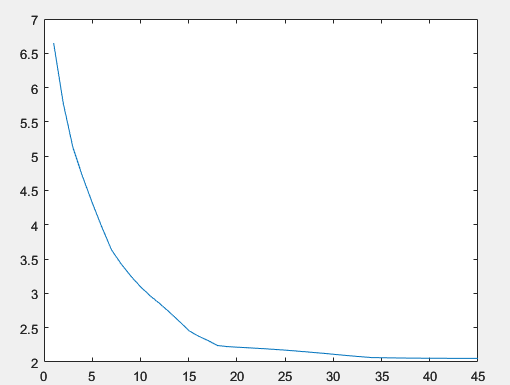
\includegraphics[width=0.5\linewidth]{Q1_2.png}
		\caption{Q1.2}
		\label{fig:Q1_2}
	\end{figure}

\end{enumerate}
	

\newpage
\section*{Problem 2 [10 pts]}
\begin{enumerate}
	\item For PCA, the loading vectors can be directly computed from the $q$ columns of  $\mU$ where  $[\mU,\mS,\mU]=svd(\mX^T\mX)$, please show that any $[\pm\vu_1,\pm\vu_2,\dots,\pm\vu_q]$ will be equivalent to $[\vu_1,\vu_2,\dots,\vu_q]$ in terms of the same variance while satisfying the orthonormality constraint. This demonstrates that if the function is nonconvex, it may have various optimal solutions, which is different from (non-trivial) convex function.
	\begin{enumerate}
		\item For orthonormality 
		\begin{align*}
			\text{When } i\neq j, \langle\pm\vu_i,\pm\vu_j\rangle = \pm  \langle\vu_i,vu_j\rangle = 0
		\end{align*}
		\item For variance
		\begin{align*}
			\|\mX\vu_i\|^2 &= \vu_i^T\mX^T\mX\vu_i \text{, s.t. }\|\vu_i\|^2=1\\
			&=trace(\vu_i^T\mX^T\mX\vu_i) = trace((-\vu_i)^T\mX^T\mX(-\vu_i))\\
			& = \|\mX(-\vu_i)\|^2
		\end{align*}
	\end{enumerate}
	\item Use the fact that $vec(\mA\mX\mB)=(\mB^T\otimes\mA)vec(\mX)$ to find the best solution to $\min\limits_{\mX} \|\mA\mX\mB-\mY\|_F^2$, where $\mA\in\R^{m\times p}, \mX\in\R^{p\times q}, \mB\in\R^{q\times n}, \mY\in\R^{m\times n}$.

	\begin{align*}
		\min\limits_{\mX} \|\mA\mX\mB-\mY\|_F^2 &= \min\limits_{\mX} \|vec(\mA\mX\mB)-vec(\mY)\|_2^2\\
		& = \min\limits_{\mX} \|(\mB^T\otimes\mA)vec(\mX)-vec(\mY)\|_2^2\\
		\text{According to the regression model: } & \min_\vx \|\mA\vx-\vy\|^2_2, \vx^* = (\mA^T\mA)^{-1}\mA^T\vy\\
		\implies vec(\mX^*) &= ((\mB^T\otimes\mA)^T(\mB^T\otimes\mA))^{-1}(\mB^T\otimes\mA)^Tvec(\mY), 
	\end{align*}

\end{enumerate}
\newpage

\section*{Problem 3 [30 pts]}
Please find \textit{USArrests} dataset online and 
\begin{enumerate}
	\item Implement your own program to reproduce the image on page 16/26 of  Dimensionality Reduction slides on Canvas.
	\begin{itemize}
		\item Fig see figure \ref{fig:q31}
		\begin{figure}
			\centering
			\fbox{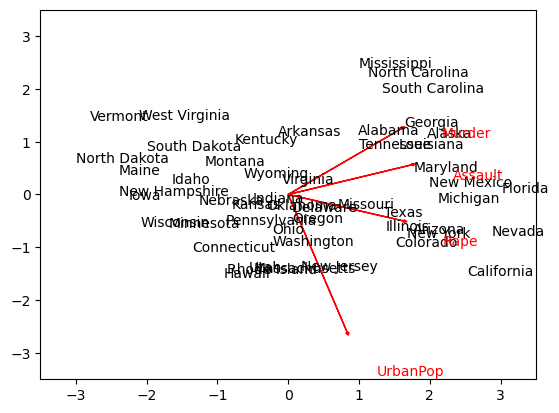
\includegraphics[width=.8\linewidth]{Q3_1.png}}
			\caption{USArrtests}
			\label{fig:q31}
		  \end{figure} 
		\item Code
		See Code \ref{code:q31}
		\mfile{Q3_1.py}\label{code:q31}
	\end{itemize}
	
	\item For each state, out of 4 features, please randomly mask one and assume it is missing (therefore you have your own $\Omega$ and $X$), please write a program following what we discussed in class (you may refer to ProximalGradientDescent.pdf on Canvas) to optimize  
		\begin{equation}
		\min_{Z} \frac{1}{2}\|P_\Omega(X-Z)\|_F^2+\|Z\|_*
	\end{equation}
\end{enumerate}


\newpage

\section*{Problem 4 [15 pts]}
Please refer to \href{https://shadow-ssml.readthedocs.io/en/latest/examples/halfmoons_example.html}{here} (for Python) or \href{https://github.com/jaejun-yoo/shallow-DANN-two-moon-dataset}{here} (for Matlab) to create a \textit{two (half) moon} dataset. Write your own \textit{spectral clustering} codes to separate the data into two groups with different colors.  You are not a allowed to call the built-in function for Python or Matlab.
\begin{enumerate}
	\item Result\\
		See Figure \ref{fig:Q4}
		\begin{figure}
			\centering
			\fbox{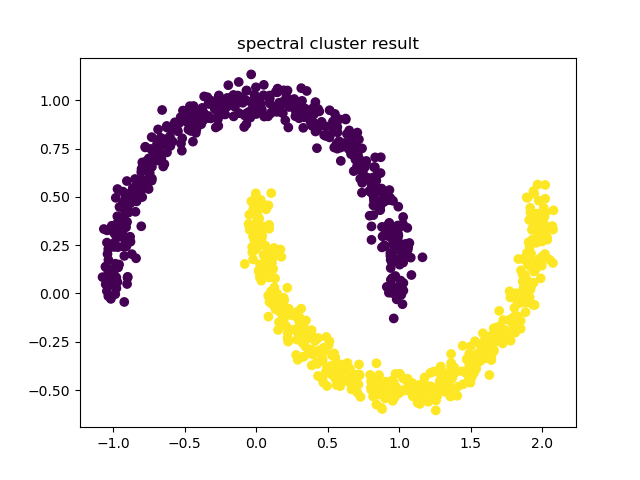
\includegraphics[width=.8\linewidth]{Q4.png}}
			\caption{Q4 Sepctral Clustering}
			\label{fig:Q4}
		  \end{figure} 
	\item Code\\
	See Code \ref{code:q4}
	\mfile{Q4.py}\label{code:q4}
	
\end{enumerate}
\newpage

\section*{Problem 5 [35 pts]}
For Logistic Regression, if the label is $\pm1$, the objective is:
\begin{equation}
\min_\vw	\sum_{i=1}^{m}log(1+exp(-y_i\vw^T\vx_i))
\end{equation}
while if the label is $\{1,0\}$ the objective is:
\begin{equation}
	\min_\vw	\sum_{i=1}^{m}log(1+exp(\vw^T\vx_i))-y_i\vw^T\vx_i
\end{equation}
\begin{enumerate}
	\item Write a program to show that the optimal solutions to the two cases  are the same by making use of gradient descent method where $m=100$ (please carefully choose the stepsize as we discussed in class). You can generate two class samples, one class's label is 1 and the other is -1 or 0 corresponding to the two formulations respectively. You can initialize $\vw$ as $\vzero$.
	\item Consider the case where class label is $\{1,0\}$ and $P(y=1|\vx,\vw)=\frac{1}{1+exp(-\vw^T\vx)}$, the maximum likelihood function is $p^y(1-p)^{1-y}$, which is equivalent to $\min -ylog(p)-(1-y)log(1-p)$, exactly the binary cross entropy. Please find optimal $p$.
	\item If we use Mean Square Error instead of cross entropy: $\min \ (y-p)^2$, and assume $y=1$ and our initial weight $\vw$ result in $p$ very close to 0, if we optimize $\vw$ by making use of gradient descent method, what will happen? Convince yourself that it will stuck at initial point and explain briefly why.
	\item For the second objective where the label is $\{1,0\}$, implement Newton method (with backtracking line search if necessary) where $m=100$.  Compare with gradient descent method and plot objective versus time consumption in one figure to observe which is faster.
	\item From now on, let's focus on the first objective where the label is $\pm1$. Please write a program to find the optimal  $\vw$ by using gradient descent method where $m=10K$, the stepsize in this case we set it as $\frac{1}{\|\mX\|_F^2}$ where each column of $\mX$ is $\vx_i$.
	\item Please write a stochastic gradient descent version for $m=10K$ (you may set the stepsize as $2/(t+1)$ where $t=1,\dots,T$ and $T=100K$) with the final output being $\bar{\vw}=\frac{1}{T}\sum_{t=1}^{T}\frac{2t}{T+1}\vw_t$.  
	\item Please compare those two methods (gradient descent vs. stochastic gradient descent) for $m=10K$ and $m=100$ by plotting objective changes versus time consumption respectively.
\end{enumerate}

\newpage
\section*{Problem 6 [15 pts]}
We consider multiclass SVM based on binary SVM. There are two options we can consider: one versus one and one versus all. Assume we have 4 classes data where each class has 2 samples: class 1 $\{\{1,0\},\{2,0\}\}$, class 2 $\{\{0,-1\},\{0,-2\}\}$, class 3 $\{\{-1,0\},\{-2,0\}\}$ and class 4 $\{\{0,1\},\{0,2\}\}$. Now use the two options (one versus one and one versus all) respectively to determine the predicted class of new data $\{0.25,1.5\}$. You should explicitly find and write each hyperplane to get full credits.

\end{document}
